\section{Polymorphism \& Interfaces}

Polymorfi betyder “mangeformet”, med hvilket der menes evnen for en variabel af type B at udgive sig for at være af type A, hvis A er en supertype til B. Fx kan klasserne Dog og Cat begge udgive sig for at være Animal objekter.

\subsection{Interfaces}

\begin{itemize}
  \item Et interface er en samling metodesignaturer. Dvs. metoder, som ingen krop har. Metoderne er ikke implementerede.
  \item En klasse kan implementere et interface, hvilket betyder, at alle interfacets metoder skal implementeres i klassen. Dette betyder, at hvis en klasse implementerer et interface, kan compileren være sikker på, at interfacets metoder eksisterer i klassen.
  \begin{itemize}
    \item Java-keyword: \verb|implements|
    \item \verb|public class Dog implements Animal { ... }|
  \end{itemize}
\end{itemize}

\subsection{Polymorfi}

\begin{itemize}
  \item Hvis en klasse implementerer et interface er klassen en subtype til interfacet. Oprettes en variabel a af type Animal kan den indeholde et objekt af en klasse som implementerer Animal interfacet, fx Dog. Nu har variablen a en formel type (Animal) og en aktuel type (Dog).
  \item Liskov’s substitutionsprincip siger, at et object af en subclass kan benyttes nårsomhelst et objekt af dens superclass forventes. Eksempelvis kan et Manager objekt altid lægges i en Employee variabel, men ikke den anden vej rundt. Da Manager objekter altid er garanteret at have samme metoder og variable (og lidt til) som Employee objekter, er dette netop muligt.
  \begin{itemize}
    \item På samme måde kan Dog objekter altid lægges i Animal variable.
  \end{itemize}
\end{itemize}

\subsection{Nedarvning}

\begin{itemize}
  \item "is-a" forhold: $<$subclass$>$ "is-a" $<$superclass$>$
  \begin{itemize}
    \item Java-keyword: \verb|extends|
    \item \verb|public class Manager extends Employee { ... }|
  \end{itemize}
  
  \item Subclasses arver alle metoder og variable fra deres superclass
  \item Subclasses kan override deres superclass' metoder, dog ikke hvis de er erklæret \verb|final|
  \begin{itemize}
    \item Polymorfi bestemmer hvilken metode der kaldes vha. objektets aktuelle type. En Employee variabel kan fx indeholde et Manager objekt (Liskov's substitutionsprincip), og polymorfien sørger for at kalde Manager-objektets overridden metode - hvis en sådan eksisterer.
    \item Override-metoder skal have samme metodesignatur (samme return type, samme parametre), som superclassen's metode.
    \item Selvom en metode er overridden kan subclasses godt kalde deres superclass' version af metoden med keywordet \verb|super|.
    \item Preconditions til overridden metoder må ikke være mere strikse end superclassens preconditions. Hvis ingen preconditions findes i superclassen må subclassens overridden metode heller ikke have preconditions.
    \item Postconditions skal omvendt være mindst ligeså strikse.
    \item En overridden metode må ikke kaste yderligere check exceptions.
  \end{itemize}
  
  \item Subclasses kan kun tilgå private variable gennem \verb|get()|-metoder, dog kan de tilgå protected variable (en slags "intern public")
  \item Nedarvning af classes betyder, at metoder og funktionalitet er tilgængelige med det samme, og principielt behøver man ikke skrive noget yderligere kode for at bruge sin nye subclass. Implementering (\verb|implements|) af interfaces betyder derimod, at man selv skal supplere koden for hver af de metoder, som interfacet definerer.
\end{itemize}

\subsection{Abstract classes}

\begin{itemize}
  \item Abstract classes er ikke instansiérbare - dvs. man kan ikke lave objekter af abstract classes. En class tagges som abstract med keywordet "abstract".\\
  Fx: \verb|public abstract class SelectableShape implements SceneShape|
  \begin{itemize}
    \item Eksempel: SelectableShape. Abstract class der implementerer SceneShape interfacet, og som definerer nogle af interfacets metoder, men ikke alle. De metoder som ikke er definerede skal derfor defineres i subclasses (fx CarShape, HouseShape).
    \item Abstract classes implementerer typisk noget af funktionaliteten i de interfaces de evt. implementerer, men ikke alt. Resten af metoderne er abstract.
    \item Fordele: Man kan lægge al ensartet funktionalitet for flere classes i én superclass, som implementerer et interface, som er nyttigt for disse classes.
    \item Ulemper: Classes kan kun extende én superclass, men implementere adskillige interfaces.
  \end{itemize}
  
  \item Refactoring - at omskrive kode så det er "bedre" eller lettere at forstå.\\
  Fx: "Extract superclass" - Lav en superclass ud fra de fælles features to eller flere classes har.
  
  \begin{center}
    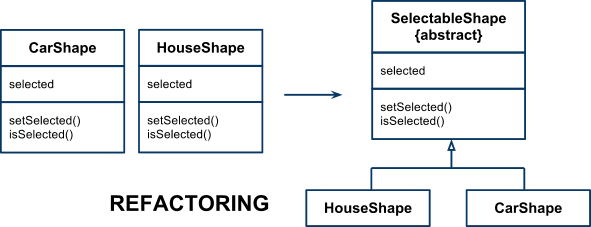
\includegraphics[scale=0.6]{images/refactor_to_template_method_pattern.png}
  \end{center}

  \begin{itemize}
    \item Refactoring adskiller sig fra design patterns idet refactoring handler om at omskrive allerede eksisterende kode, mens design patterns handler om at planlægge sit arbejde så man kan undgå at skulle benytte sig af refactoring.
  \end{itemize}

  \item Template method - en metode som flyttes fra subclasses til en superclass, og som kalder primitive operations, som kan være forskellige, i subclasses.
  \begin{itemize}
    \item Design pattern
    \item En \verb|templateMethod()| er en metode i en abstract class, som kalder abstract methods (dvs metoder som bliver defineret af subclasses som extender denne abstract class). Altså er en \verb|templateMethod()| en metode, som kalder andre metoder, som ikke endnu er blevet defineret.
    \item Eksempel: \verb|drawSelection()| i SelectableShape - \verb|drawSelection()| er defineret i SelectableShape, men kalder metoder \verb|draw()| og \verb|translate()|, som er abstract methods i SelectableShape, men som bliver defineret i CarShape og HouseShape.
  \end{itemize}

  \begin{center}
    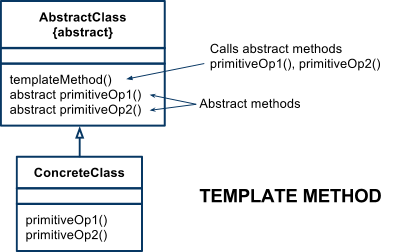
\includegraphics[scale=0.7]{images/template_method_pattern.png}
  \end{center}

\end{itemize}





